\documentclass[12pt]{report}
\usepackage[parfill]{parskip}
\usepackage[utf8]{inputenc}
\usepackage{graphicx}
\usepackage{amsthm}
\usepackage{amsmath}
\usepackage{amsfonts}
\usepackage{braket}
\usepackage{mathtools}
\usepackage{cancel}
\usepackage[dvipsnames]{xcolor}
\usepackage{hyperref}
\usepackage{todonotes}
\usepackage[capitalize]{cleveref}
\usepackage[section]{placeins}

\usetikzlibrary{decorations.markings,math,calc}

\creflabelformat{equation}{#2\textup{#1}#3}
\Crefname{equation}{Eqn.}{Eqns.}
\Crefname{figure}{Figure}{Figures}
\newcommand{\crefrangeconjunction}{--}

% \usepackage{commands}

\graphicspath{ {figures/} }
% \FloatBarrier

\title{
{Title}\\
% {\large A Thesis \\presented to \\ the Faculty of California Polytechnic State University, \\San Luis Obispo}\\
}
\author{Max Varverakis}
\date{\today}

\newtheorem{theorem}{Theorem}[chapter]
\newtheorem{corollary}{Corollary}[theorem]
\newtheorem{lemma}[theorem]{Lemma}

\theoremstyle{definition}
\newtheorem{definition}{Definition}[chapter]
\newtheorem{example}{Example}[chapter]
% customize end of example symbol
% \AtBeginEnvironment{example}{%
%     \pushQED{\qed}\renewcommand{\qedsymbol}{$\triangle$}%
% }
% \AtEndEnvironment{example}{\popQED\endexample}

\renewcommand{\bibname}{References}

\includeonly{
    % chapters/Rep_Theory_Background, 
    % chapters/Top_Background, 
    chapters/The_Braid_Group,
    % chapters/tikz_test
}

\begin{document}

% load custom commands (placed after begin document so that VSCode intellisence recognizes the commands)
\newcommand{\ehat}{\hat{e}}
\newcommand{\mat}[3]{{{#1}^#2}_#3}
\newcommand{\sotwo}{\textrm{SO}{(2)}}
\newcommand{\C}{\mathbb{C}}
\newcommand{\R}{\mathbb{R}}
\newcommand{\Z}{\mathbb{Z}}
\newcommand{\D}{\mathbb{D}}
\newcommand{\Q}{\mathbb{Q}}
\newcommand{\iv}[1]{{ #1 }^{-1}}
\newcommand{\aut}[1]{\textrm{Aut}\!\left( #1 \right)}
\newcommand{\iso}{\simeq}
\newcommand{\niso}{\not\simeq}
\newcommand{\st}{~\big|~}
\newcommand{\tr}[1]{\textrm{tr}\left(#1\right)}
\newcommand{\size}[1]{\left|#1\right|}
\newcommand{\sheet}[2]{\widetilde{#1}_{#2}}
% \newcommand{\ra}{\right\rangle}
% \newcommand{\la}{\left\langle}
% \newcommand{\lra}[1]{\la{#1}\ra}


% \renewcommand{\vec}[1]{\mathbf{#1}} % Uncomment to use bold vectors
\newcommand{\vd}[1]{\dot{\vec{#1}}}

\maketitle

\tableofcontents

\chapter{Representation Theory Background}\label{ch:rep_background}

\begin{definition}[Representations of a Group]
    If there is a homomorphism from a group $G$ to a group of operators $U(G)$ on a linear vector space $V$, we say that $U(G)$ forms a \textit{representation} of $G$ with dimension $\dim V$.
\end{definition}

The representation is a map
\begin{equation}
    g\in G\xrightarrow{U} U(g)
\end{equation}
in which $U(g)$ is an operator on the vector space $V$. For a set of basis vectors $\{\hat{e_i},i=1,2,\dots,n\}$, we can realize each operator $U(g)$ as an $n\times n$ matrix $D(g)$.
\begin{equation}
    U(g)\ket{e_i} = \sum_{j=1}^n \ket{e_j}{{D(g)}^j}_i = \ket{e_j}{{D(g)}^j}_i,
\end{equation}
where the first index $j$ is the row index and the second index $i$ is the column index. We use the Einstein summation convention, so repeated indices are summed over. Note that the operator multiplication is defined as
\begin{equation}
    U(g_1)U(g_2) = U(g_1g_2),
\end{equation}
which satisfies the group multiplication rules.

\begin{definition}
    If the homomorphism defining the representation is an isomorphism, then the representation is \textit{faithful}. Otherwise, it is \textit{degenerate}.
\end{definition}

\begin{example}
    Let $G$ be the group of continuous rotations in the $xy$-plane about the origin. We can write $G = \{R(\phi),0\leq\phi\leq2\pi\}$ with group operation $R(\phi_1)R(\phi_2) = R(\phi_1+\phi_2)$. Consider the 2-dimensional Euclidean vector space $V_2$. Then we define a representation of $G$ on $V_2$ by the familiar rotation operation
    \begin{align}
        \hat{e}_1' &= U(\phi)\hat{e}_1 = \hat{e}_1\cdot\cos\phi + \hat{e}_2\cdot\sin\phi\\
        \hat{e}_2' &= U(\phi)\hat{e}_2 = -\hat{e}_1\cdot\sin\phi + \hat{e}_2\cdot\cos\phi.
    \end{align}
This gives us the matrix representation
\begin{equation}
    D(\phi) = \begin{pmatrix}
        \cos\phi & -\sin\phi\\
        \sin\phi & \cos\phi
    \end{pmatrix}.
\end{equation}
To further illustrate this representation, if we consider an arbitrary vector $\hat{e_i}x^i=\vec{x}\in V_2$, then we have
\begin{equation}
    \vec{x}' = U(\phi)\vec{x} = \hat{e}_j{x'}^j,
\end{equation}
where ${x'}^j = {{D(\phi)}^j}_i x^i$.
\end{example}

\begin{definition}[Equivalence of Representations]
    For a group $G$, two representations are \textit{equivalent} if they are related by a similarity transformation. Equivalent representations form an equivalence class.
\end{definition}

To determine whether two representations belong to the same equivalence class, we define
\begin{definition}[Characters of a Representation]
    The \textit{character} $\chi(g)$ of an element $g\in G$ in a representation $U(g)$ is defined as $\chi(g) = \text{Tr}~D(g)$.
\end{definition}
Since trace is independent of basis, the character serves as a class label.

Vector space representations of a group have familiar substructures, which are useful in constructing representations of the group.
\begin{definition}[Invariant Subspace]
    Let $U(G)$ be a representation of $G$ on a vector space $V$, and $W$ a subspace of $V$ such that $U(g)\ket{x}\in W$ for all $\vec{x}\in W$ and $g\in G$. Then $W$ is an \textit{invariant subspace} of $V$ with respect to $U(G)$. An invariant subspace is \textit{minimal} or \textit{proper} if it does not contain any non-trivial invariant subspace with respect to $U(G)$.
\end{definition}

The identification of invariant subspaces on vector space representations leads to the following distinction of the representations.
\begin{definition}[Irreducible Representation]
    A representation $U(G)$ on $V$ is \textit{irreducible} if there is no non-trivial invariant subspace in $V$ with respect to $U(G)$. Otherwise, it is \textit{reducible}. If $U(G)$ is reducible and its orthogonal complement to the invariant subspace is also invariant with respect to $U(G)$, then the representation is \textit{fully reducible}.
\end{definition}

\begin{example}
    Under the group of 2-dimensional rotations, consider the 1-dimensional subspace spanned by $\ehat_1$. This subspace is not invariant under 2-dimensional rotations, because a rotation of $\ehat_1$ by $\pi/2$ results in the vector $\ehat_2$ that is clearly not in the subspace spanned by $\ehat_1$. A similar argument shows that the subspace spanned by $\ehat_2$ is not invariant under 2-dimensional rotations.

    However, consider the linear combination of basis vectors
    \begin{equation}
        \ehat_\pm = \frac{1}{\sqrt{2}}\left( \mp\ehat_1 + i\ehat_2 \right),
    \end{equation}
    where $i = \sqrt{-1}$. Then a rotation by angle $\phi$, denoted in operator form as $U(\phi)$, acts on $\ehat_\pm$ by
    \begin{align}
        U(\phi)\ket{\ehat_+} &= U(\phi)\frac{1}{\sqrt{2}}(-\ehat_1 + i\ehat_2) \\
        &= \frac{1}{\sqrt{2}}(-U(\phi)\ket{\ehat_1} + iU(\phi)\ket{\ehat_2}) \nonumber \\
        &= \frac{1}{\sqrt{2}}\left( -\ehat_1\cos\phi - \ehat_2\sin\phi -i\ehat_1\sin\phi + i\ehat_2\cos\phi \right) \nonumber \\
        &= \frac{1}{\sqrt{2}}\left( -\ehat_1(\cos\phi+ i\sin\phi) +i\ehat_2(\cos\phi-i\sin\phi) \right) \nonumber \\
        % &= \frac{1}{\sqrt{2}}\big(\ehat_1(-\cos\phi+i\sin\phi) + \ehat_2(i\cos\phi + \sin\phi)\big) \nonumber \\
        % &= \frac{1}{\sqrt{2}}(-\ehat_1 + i\ehat_2)(\cos\phi - i\sin\phi) \nonumber \\
        & \colorbox{red}{\textbf{Not Done}} \nonumber \\
        &= \ehat_+ (\cos\phi - i\sin\phi) \nonumber \\
        &= \ehat_+ e^{-i\phi}, \\
        \textrm{and } U(\phi)\ket{\ehat_-} &= \ehat_- e^{i\phi}.
    \end{align}

\end{example}



The irreducible representation matrices satisfy \colorbox{red}{orthonormality and completeness} relations.\textbf{ Thm. 3.5}?

\begin{example}[Generator of $\sotwo$]
    Consider the rotations of a 2-dimensional Euclidean vector space about the origin. Let $\ehat_1$ and $\ehat_2$ be orthonormal basis vectors of this space. Using geometry, we can determine how a rotation by some angle $\phi$, written in operator form as $R(\phi)$, acts on the basis vectors:
    \begin{align}
        R(\phi)\ehat_1 &= \ehat_1\cos\phi + \ehat_2\sin\phi \label{eq:rot_1}\\
        R(\phi)\ehat_2 &= -\ehat_1\sin\phi + \ehat_2\cos\phi.\label{eq:rot_2}
    \end{align}
    In matrix form, we can write
    \begin{equation}
        R(\phi) = 
        \begin{pmatrix}
            \cos\phi & -\sin\phi \\
            \sin\phi & \cos\phi
        \end{pmatrix}
    \end{equation}
    which allows us to write \cref{eq:rot_1,eq:rot_2} in a condensed form
    \begin{equation}
        R(\phi)\ehat_i = \ehat_j{{R(\phi)}^j}_i,
    \end{equation}
    where we are summing over $j=1,2$.

    Now, let $\vec{x}$ be an arbitrary vector in the plane. Then $\vec{x}$ has components $x^i$ in the basis $\{\ehat_i\}$, where $i=1,2$. Equivalently, we can write $\vec{x}=\ehat_i x^i$. Then under rotations, $\vec{x}$ transforms in accordance to the basis vectors
    \begin{align}
        R(\phi)\vec{x} &= R(\phi)\ehat_i x^i \label{eq:rot_vec} \\
        &= \ehat_j{{R(\phi)}^j}_i x^i \nonumber \\
        &= \left( \ehat_1\mat{R(\phi)}{1}{i} + \ehat_2\mat{R(\phi)}{2}{i} \right)x^i \nonumber \\
        &= \left( \ehat_1\cos\phi + \ehat_2\sin\phi \right) x^1 + \left( \ehat_1(-\sin\phi) + \ehat_2\cos\phi \right) x^2 \nonumber \\
        &= \left( x^1\cos\phi - x^2\sin\phi \right)\ehat_1 + \left( x^1\sin\phi + x^2\cos\phi \right)\ehat_2.  \nonumber
    \end{align}

    Observe that $R(\phi)R^\top(\phi) = E$ where $E$ is the identity matrix. This is precisely what defines \textit{orthogonal matrices}. For 2-dimensional vectors in the plane, it is clear that these rotations do not change the length of said vectors. This can be verified by using \cref{eq:rot_vec}:
    \begin{align}
        |R(\phi)\vec{x}|^2 &= |\ehat_j\mat{R(\phi)}{j}{i} x^i|^2 \\
        &= \left|\left( x^1\cos\phi - x^2\sin\phi \right)\ehat_1 + \left( x^1\sin\phi + x^2\cos\phi \right)\ehat_2\right|^2 \nonumber \\
        &= {\left( x^1\cos\phi - x^2\sin\phi \right)}^2 + {\left( x^1\sin\phi + x^2\cos\phi \right)}^2 \nonumber \\
        &= \left( \cos^2\phi + \sin^2\phi \right)x^1 x_1 + \left( \sin^2\phi + \cos^2\phi \right)x^2 x_2 \nonumber \\
        &= x^1 x_1 + x^2 x_2 = |\vec{x}|^2. \nonumber
    \end{align}

    Similarly, notice that for any continuous rotation by angle $\phi$, $\det R(\phi) = \cos^2\phi+\sin^2\phi = 1$. In general, orthogonal matrices have determinant equal to $\pm1$. However, the result of the above determinant of $R(\phi)$ implies that all continuous rotations in the 2-dimensional plane have determinant equal to $+1$. These are the \textit{special orthogonal matrices of rank 2}. This family of matrices is denoted $\sotwo$. Furthermore, there is a one-to-one correspondence with $\sotwo$ matrices and rotations in a plane.

    We define the group of continuous rotations in a plane by letting $R(0) = E$ be the identity element corresponding to no rotation (i.e., a rotation by angle $\phi=0$), and defining the inverse of a rotation as $R^{-1}(\phi) = R(-\phi) = R(2\pi-\phi)$. This group can be called the $\sotwo$ group. Lastly, we define group multiplication as $R(\phi_1)R(\phi_2) = R(\phi_1+\phi_2)$ and note that $R(\phi) = R(\phi\pm2\pi)$, which can be verified geometrically. Thus, group elements of $\sotwo$ can be labelled by the angle of rotation $\phi\in[0,2\pi)$.

    Now we can find a generator of $sotwo$ by considering an infinitesimal rotation, labelled by some infinitesimal angle $d\phi$. Then this is equivalent to the identity plus some small rotation, which we can write as
    \begin{equation}
        R(\textrm{d}\phi) = E - i \textrm{d}\phi J
    \end{equation}
    where the scalar quantity $-i$ is introduced for later convenience and $J$ is some quantity independent of the rotation angle. If we consider the rotation $R(\phi + \textrm{d}\phi)$, then there are two equivalent ways to interpret this rotation
    \begin{align}
        R(\phi + \textrm{d}\phi) &= R(\phi)R(\textrm{d}\phi) = R(\phi)(E - i \textrm{d}\phi J) = R(\phi) - i \textrm{d}\phi R(\phi)J \\
        R(\phi + \textrm{d}\phi) &= R(\phi) + \textrm{d}R(\phi) = R(\phi) + \textrm{d}\phi\frac{\textrm{d}R(\phi)}{\textrm{d}\phi}
    \end{align}
    where the second equation can be thought of as a Taylor expansion of $R(\phi + \textrm{d}\phi)$ about $\phi$. Equating the two expressions for $R(\phi + \textrm{d}\phi)$ yields
    \begin{equation}
        \textrm{d}R(\phi) = -i\textrm{d}\phi R(\phi)J.
    \end{equation}
    Solving this differential equation (with boundary condition $R(0)=E$) provides us with an equation for any group element involving $J$:
    \begin{equation}
        R(\phi) = e^{-i\phi J},
    \end{equation}
    where $J$ is called the \textit{generator} of the group.
\end{example}

\chapter{Relevant topological definitions}\label{ch:top_background}

The braid group is formally defined in terms of topology. In order to understand the braid group, we must first understand the underlying topological properties that are used to define the braid group. The following is a brief introduction to the relevant topological concepts~\cite{Fulton1997,Kassel2008}.

Similar to an isomorphism in algebra, the notion of topological equivalence is given by the following definition.
\begin{definition}
    Consider $X$ and $Y$ to be two topological spaces. A \textit{homotopy} between two continuous functions $f,g:X\to Y$ is a continuous function $H:X\times[0,1]\to Y$ such that $H(x,0)=f(x)$ and $H(x,1)=g(x)$ for all $x\in X$. If such a homotopy exists, we say that $f$ and $g$ are \textit{homotopic}.
\end{definition}
The homotopy $H$ can be thought of as a continuous deformation of $f$ into $g$. The interval $\left[ 0,1 \right]$ represents the ``time'' parameter of the deformation. At time equal to 0, the function $H$ is equal to $f$, and at time equal to 1, the function $H$ is equal to $g$. If two functions are homotopic, then they belong to the same homotopy class, which is an equivalence class of functions under the relation of homotopy.

\begin{definition}
    A \textit{loop} on a topological space $X$ is a continuous function $\ell:[0,1]\to X$ such that $\ell(0) = \ell(1)$. In other words, the path of $\ell$ starts and ends at the same point in $X$. Often, this point is called the \textit{base point} of the loop.
\end{definition}

Equipped with the above definitions, the equivalence of loops on a topological space is defined as follows.
\begin{definition}
    A \textit{homotopy class of loops} on a topological space $X$ is an equivalence class of loops under the relation of homotopy. Simply put, a homotopy of loops is a continuous transformation of one loop into another. If two loops $\ell_1,\ell_2:[0,1]\to X$ with base point $\xi\in X$ are homotopic, then there exists a continuous map $H:[0,1]\times [0,1]\to X$ such that:
    \begin{enumerate}
        \item $H(0,t) = \xi = H(1,t)$ for all $t\in [0,1]$, and
        \item $H(s,0) = \ell_1(s)$ and $H(s,1) = \ell_2(s)$ for all $s\in [0,1]$.
    \end{enumerate}
    Property 1 ensures that the starting/ending point of the loop remains fixed throughout the deformation from $\ell_1$ to $\ell_2$, and property 2 follows from the definition of a homotopy.
\end{definition}

\begin{definition}
    The \textit{fundamental group} of a topological space $X$ with base point $\xi$ is defined as the collection of loops on $X$ with base point $\xi$ modulo homotopy. In other words, the fundamental group is the collection of equivalence classes of loops under homotopy. This is written as
    \begin{align*}
        \pi(X,\xi):=\left\{ \textrm{loops }\ell \textrm{ on }X \textrm{ with base point }\xi \right\}/\textrm{homotopy}.
    \end{align*}
    Often times, the base point of a loop is arbitrary, so we can write $\pi(X)$ instead of $\pi(X,\xi)$ to denote the fundamental group of $X$.
\end{definition}

The group structure of the fundamental group is defined as operations on the loops themselves. Consider two loops $\ell_1,\ell_2:[0,1]\to X$ with base point $\xi$. Then the product $\ell_1\cdot\ell_2$ is defined in terms of \textit{concatenation} of the two loops. Specifically, this defines a new loop $(\ell_1\cdot\ell_2)(t)=\mathcal{L}(t):[0,1]\to X$ where $\mathcal{L}(t) = \ell_1(2t)$ on $\left[ 0,\frac{1}{2} \right]$ and $\mathcal{L}(t) = \ell_2(2t-1)$ on $\left[ \frac{1}{2},1 \right]$. Loop concatenation can be thought of as stitching the loops together at the shared base point. As $t$ ranges from 0 to 1, we can think of the first half of the deformation as traversing the first loop at twice the original speed and then traveling along the second loop at twice the original speed in the second half of the deformation.

In the above description, note that each group element $\ell$ is actually an equivalence class of loops $\left[ \ell \right]$ under the relation of homotopy. So the concatenation of two loops $\ell_1$ and $\ell_2$ is really the concatenation of any two loops belonging to the equivalence classes $\left[ \ell_1 \right]$ and $\left[ \ell_2 \right]$, which becomes the equivalence class $\left[ \ell_1\cdot\ell_2 \right]$.

In the fundamental group, the inverse of an element is the identical topological path traversed in the opposite direction. If $\gamma:[0,1]\to X$ is a loop on $X$, then $\iv{\gamma}(t) \coloneq \gamma(1-t)$.

% \begin{example}
%     Consider a \textbf{3-dimensional(?)} torus $T^3$. The fundamental group of the torus is $\pi(T^3)$. There are two types of loops on the torus: those that pass through the hole of the torus, and those that do not.
% \end{example}

Just as how homotopy describes a continuous transformation from one continuous path on a topological space to another, topological equivalence is established in a broader sense in the following definition.
\begin{definition}
    A continuous, bijective function $f:X\to Y$ between two topological spaces $X$ and $Y$ such that the inverse $\iv{f}:Y\to X$ is also continuous and bijective is called a \textit{homeomorphism}. If there exists such a homeomorphism, then we say $X$ is \textit{homeomorphic} to $Y$. Moreover, an \textit{embedding} of topological spaces is a continuous function that is a homeomorphism when restricted to its image. If we have a continuous family of homeomorphisms $f_t:X\to Y$ for $t\in[0,1]$, then we say that $X$ and $Y$ are \textit{isotopic}. The isotopy of $X$ and $Y$ can be written as a function $H:X\times[0,1]\to Y$ such that
    \begin{enumerate}
        \item $H(x,0)=x$ for all $x\in X$, 
        \item $H(x,1)=f(x)$ for all $x\in X$, and
        \item $H(-,t)$ is an embedding of $X$ onto $Y$ for all $t\in[0,1]$.
    \end{enumerate}
\end{definition}
Evidently, isotopy defines a stronger and more broad notion of topological equivalence, which will be important in defining representations of the braid group.

\chapter{The Braid Group}\label{ch:braid_group}

\begin{definition}
    The \textit{configuration space} of $n$ ordered distinct points in the complex plane $\C$ is defined as $M_n = \left\{ \left( z_1,\dots,z_n \right)\in\C ; z_i\neq z_j,\forall i\neq j \right\}$. Alternatively, consider $\mathcal{D}$ to be the collection of all hyperplanes $H_{i,j}=\left\{ z_i=z_j \right\}\in\C^n$ for $1\leq i < j \leq n$. Then we can define $M_n = \C^n \setminus \mathcal{D}$.
\end{definition}

Note that $\left( z_1,z_2,z_3,\dots,z_n \right)$ and $\left( z_2,z_1,z_3,\dots,z_n \right)$ are different points in the configuration space $M_n$. Before studying the various interpretations of the braid group, we first define the braid group itself.

\begin{definition}
    The \textit{pure braid group} on $n$ strands, denoted $PB_n$, is the fundamental group of $M_n$. One can write $PB_n = \pi_1(M_n)$.
\end{definition}

\section{Visualization of pure braids}

We can think of a pure braid as a loop in $M_n$:
\begin{align*}
    \beta : \left[ 0,1 \right] &\to M_n \\
    t &\mapsto \beta(t) = \left( \beta_1(t),\beta_2(t),\dots,\beta_n(t) \right),
\end{align*}
with some base point. Conventionally, we define the base point as the $n$-tuple of integers $(1,2,3,\dots,n)\in \C^n$. Then a pure braid can be though of the motion of these points in the complex plane as $t$ ranges from 0 to 1 in which $\beta_i(t)$ is defined and $\beta_i(t)\neq \beta_j(t)$ for every $t\in[0,1]$ and $i\neq j\in\left\{ 1,2,\dots,n \right\}$. Because each $\beta_i$ is a loop, it must start and end at the point $i$ (e.g., $\beta_i(0)=\beta_i(1)=i$). Recall that the loops are actually equivalence classes of loops under homotopy. As a result, we can continuously deform the motion of the $n$ points while maintaining the same pure braid (up to equivalence) so long as we preserve the pairwise distinction of the points for all time $t\in[0,1]$.

A common visualization of pure braids is to plot the motion of the points in 3-dimensional space. For each $t\in [0,1]$, we draw the points $\left( \beta_i(t),t \right)$ in $\C\times[0,1]$ for every $i\in\left\{ 1,\dots,n \right\}$. The space $\C\times[0,1]$ can be thought of as a spacetime diagram, where the motion of the points is plotted in the complex plane at each time $t$, with the time being the vertical axis. The convention is to have $\C\times\left\{ 0 \right\}$ placed above $\C\times\left\{ 1 \right\}$, so that the motion of the points is plotted from top to bottom.

\missingfigure[figwidth=6cm]{Gonzalez Figure 1}

For every $i\in\left\{ 1,\dots,n \right\}$, the motion of a single point starting at $(i,0)$ and ending at $(i,1)$ is known as the $i$-th \textit{strand} of the pure braid. This can also be described by the $i$-th projection of the $n$-tuple $\beta(t)$. Thus, two braids are equivalent under homotopy if, for every moment of a continuous deformation of the $n$ strands in $\C\times [0,1]$, the (fixed) endpoints $((1,0),(2,0),\dots,(n,0))$ and $((1,1),(2,1),\dots,(n,1))$ are connected by strands that are pairwise disjoint where each strand intersects the plane $\C\times\left\{ t \right\}$ exactly once for every $t\in[0,1]$.

As pure braids are members of the pure braid group, multiplication is a well-defined operation. In the context of $M_n$, multiplication of pure braids involves the concatenation of loops. Visually, this is the process of stacking braids on top of each other, and then rescaling the time dimension so that $t$ ranges from 0 to 1.

\section{General braids}
In the previous section, we defined pure braids in which the endpoints of each strand are identical at the beginning and end of the motion. This notion generalizes to define (non-pure) braids. First, we define a more general configuration space than $M_n$. The symmetric group $S_n$ permutes the $n$ distinct points in $\C$. Then the \textit{configuration space of n unordered points in $\C$} is the quotient space $N_n = M_n/S_n$.

\begin{definition}
    The braid group on $n$ strands is the fundamental group of $N_n$, denoted $B_n = \pi_1(N_n)$.
\end{definition}

The visualization of a braid is the same as in the case of pure braids, only now the endpoints of each strand do not necessarily match the starting points. For example, the $i$-th strand may start at the point $(i,0)$ but end at the point $(j,1)$ for $i,j\in\left\{ 1,\dots,n \right\}$. The equivalence of strands is still defined as before under the homotopy of loops. Loop concatenation defines the multiplication of braids, as before.

\section{Standard generators of the braid group}\label{sec:std_gens}
Originally proposed by Artin~\cite{Artin1947}, each braid can be decomposed into a product of \textit{standard generators} of the braid group. When visualizing braids in $\R\times[0,1]$, a crossing of two strands is clearly indicated by one going over the other. Suppose each crossing occurs at a different time $t\in[0,1]$. Then by rescaling the time component of an arbitrary braid, we can deconstruct it into a stack of simple braids with only one crossing between neighboring strands per braid. Each single crossing of strands can be obtained by performing a transposition between neighboring endpoints of the strands.

\missingfigure[figwidth=6cm]{Gonzalez Figure 2}

For instance, swapping the endpoints of the $i$-th and $(i+1)$-th strands can be written as applying $\sigma_i$ to the identity braid (i.e., the braid that starts without any crossings of strands). It must be noted that there are two distinct ways to swap the endpoints of two strands. From a top-down perspective looking at the plane $\C\times\left\{ t \right\}$ for some time $t$, $\sigma_i$ swaps $(i,t)$ and $(i+1,t)$ in a clockwise rotation. The reverse of this operation (i.e., twisting the endpoints around in the counterclockwise direction) is denoted $\sigma_i^{-1}$. The standard generators of the braid group $B_n$ are defined as the set $\left\{ \sigma_1,\sigma_2,\dots,\sigma_{n-1} \right\}$. An arbitrary braid can be constructed by concatenating (or stacking) the simple braids made from the standard generators before rescaling the time coordinate to $[0,1]$.

\section{Automorphisms of the free group}\label{sec:Aut_Fn}

Consider the $n$-times punctured disk $\D_n$. The fundamental group of $\D_n$ involves loops that start and end at the same (fixed) base point in $\partial\D_n$. Up to homotopy, a clockwise-directional loop that encompasses the $i$-th hole in $\D_n$ corresponds to the $i$-th generator of the free group $F_n$ of rank $n$, which is illustrated in \cref{fig:Gen_on_Dn}. In fact, $\pi_1\left( \D_n \right) = F_n$. This equality allows us to define a representation of the braid group on $n$ strands as automorphisms of $F_n$.

\begin{figure}[htbp]
    \centering
    % Suggested circle radius >= 3 cm
% \usetikzlibrary{decorations.markings}
\def\circleRadius{3cm}
\def\sep{\circleRadius*0.175}

\newcommand{\drawloop}[3]{\draw[ultra thick, postaction={decorate}] (0,-\circleRadius) .. controls #1 .. node[pos=#3, left] {#2} (.0*\sep,-\circleRadius);}

\begin{tikzpicture}[decoration={markings, 
	mark= at position 0.75 with {\arrow{latex},sloped}}
] 
        \node[anchor=north west, font=\Large] at (-\circleRadius, \circleRadius) {$\D_n$};

        \draw[ultra thick] (0,0) circle (\circleRadius);
        \filldraw [black] 
                        (-\circleRadius + \sep,0) circle (2pt) node[above, yshift=.2*\sep] {$1$}
                        (\circleRadius - \sep,0) circle (2pt) node[above, yshift=.2*\sep] {$n$}
                        (0,0) circle (2pt) node[above, yshift=.2*\sep] {$i$};
        \path (-\circleRadius/2 + \sep/2,0) node {$\scalebox{1.5}{$\cdots$}$};
        \path (\circleRadius/2 - \sep/2,0) node {$\scalebox{1.5}{$\cdots$}$};

        \drawloop{(-.35*\circleRadius,0.4*\circleRadius) and  (.35*\circleRadius,0.4*\circleRadius)}{$x_i$}{.2}

        \drawloop{(-1.6*\circleRadius,0.37*\circleRadius) and  (-.65*\circleRadius,0.43*\circleRadius)}{$x_1$}{.1}
        
        \drawloop{(.65*\circleRadius,0.43*\circleRadius) and  (1.6*\circleRadius,0.37*\circleRadius)}{$x_n$}{.25}
        
        % base point for loop/arrow
        \filldraw [red] (0,-\circleRadius) circle (2pt);
\end{tikzpicture}

    \caption{For each $i\in\left\{ 1,\dots,n \right\}$, the clockwise-directional loop encircling the $i$-th hole in $\D_n$ corresponds to the $i$-th free generator of $F_n$ (i.e., $x_i$). The red dot indicates the (arbitrary) base point for the loops in $\pi_1(\D_n)$.}\label{fig:Gen_on_Dn}
\end{figure}

Each braid $\beta\in B_n$ is realized as an automorphism of $\pi_1(\D_n) = F_n$ (up to isotopy) where each loop $\gamma\in\pi_1(\D_n)$ is sent to another loop $\beta(\gamma)$. In other words, we have a representation of the braid group defined by
\begin{align}
    \rho: B_n &\to \aut{F_n} \\
    \beta &\mapsto \rho_\beta.
\end{align}
The action of $\beta$ on a loop $\gamma$ is defined by the rearrangements of the $n$ holes in $\D_n$, similar to the action of the standard generators of $B_n$ on the base points in $\C\times\left\{ 1 \right\}$. In terms of the standard generators of $B_n$, each $\sigma_i$ corresponds to switching the places of hole $i$ and hole $i+1$ by means of a clockwise rotation, as seen in \cref{fig:sigma_on_Dn}. This is identical to viewing the action of $\sigma_i$ on the base points (\cref{sec:std_gens}) from above, looking down on the $\C\times\left\{ t \right\}$-plane. As before, the inverse action $\iv{\sigma_i}$ is a counterclockwise rotation of the two adjacent holes $i$ and $i+1$ in $\D_n$. These actions respect the group operation of loop concatenation.

\colorbox{red}{A note on convention of directions/consistency up to inverses.}

% \begin{figure}[htbp]
%     \centering
%     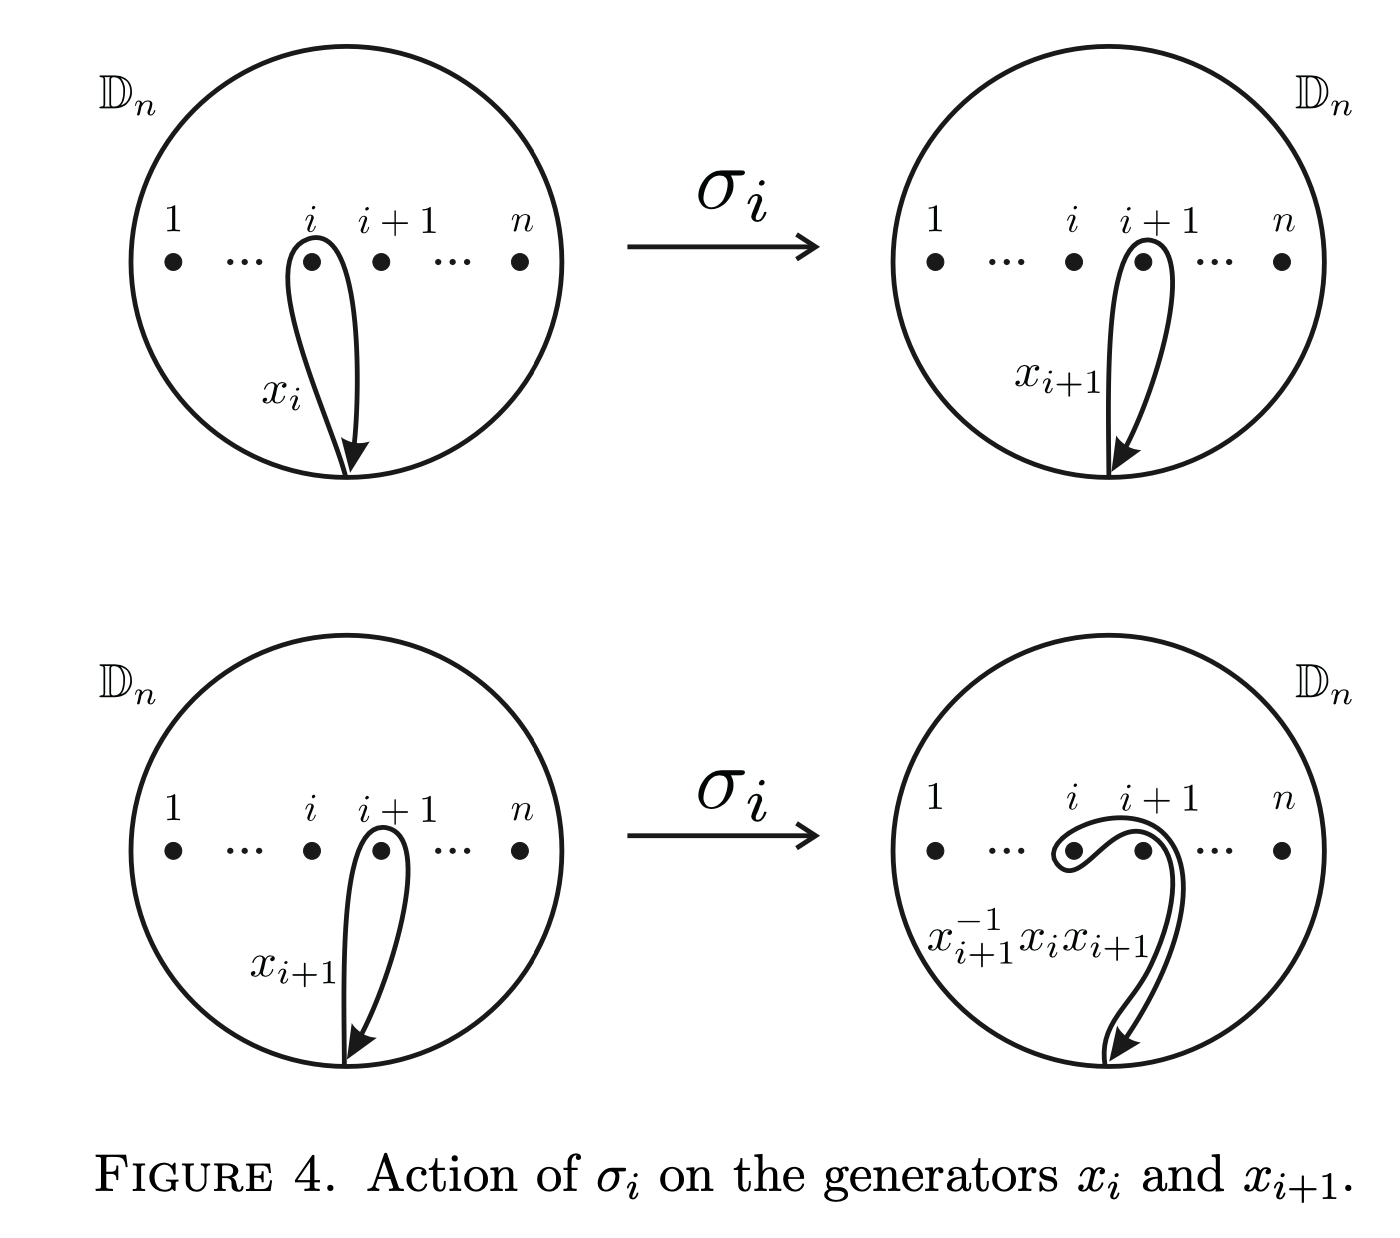
\includegraphics[width = .5\textwidth]{Gonzalez_Fig4_sigma_on_Dn.png}
%     \caption{\colorbox{red}{Gonzalez Figure 4}}\label{fig:sigma_on_Dn}
% \end{figure}

\begin{figure}[htbp]
    \centering
    \def\circleRadius{2.5cm}
\def\sep{\circleRadius*0.175}
\def\XOff{1.5*\circleRadius}
\def\YOff{-2.5*\circleRadius}

\pgfdeclarelayer{edgelayer}
\pgfdeclarelayer{nodelayer}
\pgfsetlayers{edgelayer,nodelayer,main}

\newcommand{\drawRegion}[3]{
        \begin{scope}[shift={#1}]
        \node[anchor=north west, font=\large] at (-\circleRadius, \circleRadius) {$\D_n$};

        \draw[ultra thick] (0,0) circle (\circleRadius);
        \filldraw [black] 
                (-\circleRadius + \sep,0) circle (2pt) node[above] {$1$}
                (\circleRadius - \sep,0) circle (2pt) node[above] {$n$}
                (-\sep,0) circle (2pt) node[above, yshift=.2*\sep] {$i$}
                (\sep,0) circle (2pt) node[above, yshift=.1*\sep] {$i+1$};
        \path (-\circleRadius/2,0) node {$\scalebox{1.5}{$\cdots$}$};
        \path (\circleRadius/2,0) node {$\scalebox{1.5}{$\cdots$}$};

        \ifx&#2&  % Check if #2 is empty
                % Do nothing if #2 is empty
        \else
                \draw[-latex, ultra thick] (0,-\circleRadius) .. controls #2 .. node[pos=0.1, left] {#3} (.05*\sep,-\circleRadius + 2.8452755906/2);
        \fi
        
        \filldraw [red] (0,-\circleRadius) circle (2pt);
        
        \end{scope}
}


\begin{tikzpicture}
        \drawRegion{(\XOff,0)}{(-1.425*\sep-.35*\circleRadius,0.39*\circleRadius) and  (-1.425*\sep+.35*\circleRadius,0.39*\circleRadius)}{$x_i$}
        
        \draw[-latex, ultra thick] (-\XOff + \circleRadius + 0.25cm, 0) -- node[above] {$\sigma_i$} (\XOff - \circleRadius - 0.25cm, 0);
        
        \drawRegion{(-\XOff,0)}{(1.3*\sep-.35*\circleRadius,0.39*\circleRadius) and  (1.3*\sep+.35*\circleRadius,0.39*\circleRadius)}{$x_{i+1}$}
        
        \drawRegion{(-\XOff,\YOff)}{(-1.425*\sep-.35*\circleRadius,0.39*\circleRadius) and  (-1.425*\sep+.35*\circleRadius,0.39*\circleRadius)}{$x_i$}

        \draw[-latex, ultra thick] (-\XOff + \circleRadius + 0.25cm, \YOff) -- node[above] {$\sigma_i$} (\XOff - \circleRadius - 0.25cm, \YOff);
        
        % \drawRegion{(\XOff,\YOff)}{}{}

        \begin{scope}[shift={(\XOff,\YOff)}]
                \node[anchor=north west, font=\large] at (-\circleRadius, \circleRadius) {$\D_n$};
        
                \draw[ultra thick] (0,0) circle (\circleRadius);
                \filldraw [black] 
                        (-\circleRadius + \sep,0) circle (2pt) node[above] {$1$}
                        (\circleRadius - \sep,0) circle (2pt) node[above] {$n$}
                        (-\sep,0) circle (2pt) node[above, yshift=.45*\sep] {$i$}
                        (\sep,0) circle (2pt) node[above, yshift=.3*\sep] {$i+1$};
                \path (-\circleRadius/2,0) node {$\scalebox{1.5}{$\cdots$}$};
                \path (\circleRadius/2,0) node {$\scalebox{1.5}{$\cdots$}$};
        
                \filldraw [red] (0,-\circleRadius) circle (2pt);

                \begin{pgfonlayer}{nodelayer}
                        \node (0) at (-1.5*\sep,.35*\sep ) {};
                        \node (1) at (0, -\circleRadius) {};
                        \node (2) at (1.5*\sep, -1.5*\sep) {$x_i x_{i+1}\iv{x_i}$};
                        \node (3) at (1.25*\sep, -.25*\sep) {};
                        \node (4) at (-.5*\sep, .35*\sep) {};
                        \node (5) at (.05*\sep, -\circleRadius + 2.8452755906/2) {};
                \end{pgfonlayer}
                \begin{pgfonlayer}{edgelayer}
                        \draw [in=105, out=-120, looseness=0.50, ultra thick] (0.center) to (1.center);
                        \draw [in=60, out=30, looseness=0.85, ultra thick] (3.center) to (0.center);
                        \draw [in=-150, out=-15, looseness=0.50, ultra thick] (4.center) to (3.center);
                        \draw [latex-, in=165, out=85, ultra thick] (5.center) to (4.center);
                \end{pgfonlayer}

                % \foreach \point in {0,1,3,4,5} {
                %         \fill[red] (\point) circle (2pt);
                %         \node[above right] at (\point) {\point};
                % }
        \end{scope}
        
        \draw[-latex, ultra thick] (-\XOff + \circleRadius + 0.25cm, 0) -- node[above] {$\sigma_i$} (\XOff - \circleRadius - 0.25cm, 0);
\end{tikzpicture}
    \caption{The action of $\sigma_i$ on the generators $x_i$ and $x_{i+1}$ as described by \cref{eq:rho_i,eq:rho_ip1,eq:rho_j}. The image of $x_i$ under $\sigma_i$ is verified visually in \cref{fig:sigma_on_x_i}}\label{fig:sigma_on_Dn}
\end{figure}

The automorphism $\rho_\beta$ is most simply defined in terms of the action of the standard generators of $B_n$ on the generators $x_1,\dots,x_n$ of $F_n$ (visualized as loops in $\D_n$). For each $i$, it follows that
\begin{align}
    &\rho_{\sigma_i}(x_{i}) = x_{i}x_{i+1} \iv{x_{i}}, \label{eq:rho_i}\\
    &\rho_{\sigma_i}(x_{i+1}) = x_{i}, \label{eq:rho_ip1}\\
    &\rho_{\sigma_i}(x_j) = x_j, \textrm{ for } j\neq i,i-1.\label{eq:rho_j}
\end{align}
Clearly, any two loops that are separated by at least one puncture will not interact while performing $\sigma_i$. The relations for adjacent loops can be verified graphically as illustrated in \cref{fig:sigma_on_Dn,fig:sigma_on_x_i}.
\begin{figure}[htbp]
    \centering
    \def\circleRadius{2.5cm}
\def\sep{\circleRadius*0.175}
\def\XOff{1.5*\circleRadius}
\def\YOff{-2.5*\circleRadius}

\usetikzlibrary{decorations.markings}

\pgfdeclarelayer{edgelayer}
\pgfdeclarelayer{nodelayer}
\pgfsetlayers{edgelayer,nodelayer,main}

\newcommand{\drawRegion}[3]{
        \begin{scope}[shift={#1}]
        \node[anchor=north west, font=\large] at (-\circleRadius, \circleRadius) {$\D_n$};

        \draw[ultra thick] (0,0) circle (\circleRadius);
        \filldraw [black] 
                (-\circleRadius + \sep,0) circle (2pt) node[above] {$0$}
                (\circleRadius - \sep,0) circle (2pt) node[above] {$n$}
                (-\sep,0) circle (2pt) node[above, yshift=.2*\sep] {$i$}
                (\sep,0) circle (2pt) node[above, yshift=.1*\sep] {$i+1$};
        \path (-\circleRadius/2,0) node {$\scalebox{1.5}{$\cdots$}$};
        \path (\circleRadius/2,0) node {$\scalebox{1.5}{$\cdots$}$};

        \filldraw [red] (0,-\circleRadius) circle (2pt);

        \ifx&#2&  % Check if #2 is empty
                % Do nothing if #2 is empty
        \else
                \draw[-latex, ultra thick] (0,-\circleRadius + 2.8452755906/2) .. controls #2 .. node[pos=0.1, left] {#3} (.05*\sep,-\circleRadius + 2.8452755906/2);
        \fi
        \end{scope}
}

\newcommand{\drawloop}[4]{\draw[ultra thick, postaction={decorate}, decoration={markings, mark= at position 0.75 with {\arrow{latex},sloped}}, #2] (0,-\circleRadius + 2.8452755906/2) .. controls #1 .. node[pos=#4, left] {#3} (.05*\sep,-\circleRadius + 2.8452755906/2);}

\newcommand{\rdrawloop}[4]{\draw[ultra thick, postaction={decorate}, decoration={markings, mark= at position 0.25 with {\arrowreversed{latex},sloped}}, #2] (0,-\circleRadius + 2.8452755906/2) .. controls #1 .. node[pos=#4, left] {#3} (.05*\sep,-\circleRadius + 2.8452755906/2);}


\begin{tikzpicture}
        \begin{scope}[shift={(-\XOff,0)}]
                \node[anchor=north west, font=\large] at (-\circleRadius, \circleRadius) {$\D_n$};
        
                \draw[ultra thick] (0,0) circle (\circleRadius);
                \filldraw [black] 
                        (-\circleRadius + \sep,0) circle (2pt) node[above] {$0$}
                        (\circleRadius - \sep,0) circle (2pt) node[above] {$n$}
                        (-\sep,0) circle (2pt) node[above, yshift=.2*\sep] {$i$}
                        (\sep,0) circle (2pt) node[above, yshift=.25*\sep] {$i+1$};
                \path (-\circleRadius/2,0) node {$\scalebox{1.5}{$\cdots$}$};
                \path (\circleRadius/2,0) node {$\scalebox{1.5}{$\cdots$}$};
        
                \filldraw [red] (0,-\circleRadius) circle (2pt);

                \begin{pgfonlayer}{nodelayer}
                        \node (0) at (.7*\sep,-.5*\circleRadius ) {};
                        \node (1) at (0, -\circleRadius + 2.8452755906/2) {};
                        \node (2) at (.5*\circleRadius, -2*\sep) {$\color{NavyBlue} x_{i+1}$};
                        \node (3) at (.9*\sep, .5*\sep) {};
                        \node (4) at (1.75*\sep, -.5*\circleRadius) {};
                        \node (5) at (.05*\sep, -\circleRadius + 2.8452755906/2) {};
                \end{pgfonlayer}
                \begin{pgfonlayer}{edgelayer}
                        \draw [in=30, out=-90, looseness=0.50, ultra thick, NavyBlue] (0.center) to (1.center);
                        \draw [in=90, out=-150, looseness=0.85, ultra thick, NavyBlue] (3.center) to (0.center);
                        \draw [in=20, out=80, looseness=0.50, ultra thick, NavyBlue, postaction={decorate}, decoration={markings, mark= at position .5 with {\arrowreversed{latex},sloped}}] (4.center) to (3.center);
                        \draw [in=-100, out=10, ultra thick, NavyBlue] (5.center) to (4.center);
                \end{pgfonlayer}
                
                % \foreach \point in {0,1,3,4,5} {
                %         \fill[red] (\point) circle (2pt);
                %         \node[above right] at (\point) {\point};
                % }

                \rdrawloop{(-1.4*\sep-.65*\circleRadius,0.7*\circleRadius) and  (-1.4*\sep+.55*\circleRadius,0.7*\circleRadius)}{purple}{$\iv{x_i}$}{.45}

                \drawloop{(-1.4*\sep-.35*\circleRadius,0.39*\circleRadius) and  (-1.4*\sep+.35*\circleRadius,0.39*\circleRadius)}{OliveGreen}{$x_i$}{.1}

        \end{scope}

        \begin{scope}[shift={(\XOff,0)}]
                \node[anchor=north west, font=\large] at (-\circleRadius, \circleRadius) {$\D_n$};
        
                \draw[ultra thick] (0,0) circle (\circleRadius);
                \filldraw [black] 
                        (-\circleRadius + \sep,0) circle (2pt) node[above] {$0$}
                        (\circleRadius - \sep,0) circle (2pt) node[above] {$n$}
                        (-\sep,0) circle (2pt) node[above, yshift=.3*\sep] {\small$i$}
                        (\sep,0) circle (2pt) node[above, xshift=0*\sep, yshift=.15*\sep] {\small$i+1$};
                \path (-\circleRadius/2,0) node {$\scalebox{1.5}{$\cdots$}$};
                \path (\circleRadius/2,0) node {$\scalebox{1.5}{$\cdots$}$};
        
                \filldraw [red] (0,-\circleRadius) circle (2pt);
                
                \begin{scope}[shift={(-.25*\sep,0)}]
                                \begin{pgfonlayer}{nodelayer}
                                \node (0) at (-1.75*\sep,-.15*\circleRadius ) {};
                                \node (1) at (.25*\sep, -\circleRadius + 2.8452755906/2) {};
                                % \node (2) at (.5*\circleRadius, -2*\sep) {$x_i x_{i+1}\iv{x_i}$};
                                \node (3) at (0*\sep, 1.5*\sep) {};
                                \node (4) at (2*\sep, -.05*\circleRadius) {};
                                \node (5) at (0*\sep, 0*\circleRadius) {};
                                \node (6) at (-1.2*\sep, .4*\sep) {};
                                \node (7) at (.3*\sep, -\circleRadius + 2.8452755906/2) {};

                                \node (ip1) at (2.5*\sep, -1.15*\sep) {$\color{NavyBlue} x_{i+1}$};
                                \node (i) at (-.4*\circleRadius, -2*\sep) {$\color{OliveGreen} x_{i}$};
                                \node (iiv) at (.1*\circleRadius, -3*\sep) {$\color{purple} \iv{x_{i}}$};
                        \end{pgfonlayer}
                        \begin{pgfonlayer}{edgelayer}
                                \draw [in=150, out=-90, looseness=0.50, ultra thick, OliveGreen] (0.center) to (1.center);
                                \draw [latex-, in=100, out=180, looseness=0.95, ultra thick, OliveGreen] (3.center) to (0.center);
                                \draw [in=0, out=90, looseness=0.9, ultra thick, NavyBlue] (4.center) to (3.center);
                                \draw [latex-, in=-100, out=-50, looseness=.9, ultra thick, NavyBlue] (5.center) to (4.center);
                                \draw [in=60, out=100, looseness=.9, ultra thick, purple] (5.center) to (6.center);
                                \draw [-latex, in=100, out=-110, looseness=.9, ultra thick, purple] (6.center) to (7.center);
                        \end{pgfonlayer}
                \end{scope}
                
                \foreach \point in {3,5} {
                                \fill[red] (\point) circle (1.5pt);
                                % \node[above right] at (\point) {\point};
                        }

                % \foreach \point in {0,1,3,4,5,6,7} {
                %         \fill[red] (\point) circle (1.5pt);
                %         \node[above right] at (\point) {\point};
                % }
        \end{scope}

        \begin{scope}[shift={(\XOff,\YOff)}]
                \node[anchor=north west, font=\large] at (-\circleRadius, \circleRadius) {$\D_n$};
        
                \draw[ultra thick] (0,0) circle (\circleRadius);
                \filldraw [black] 
                        (-\circleRadius + \sep,0) circle (2pt) node[above] {$0$}
                        (\circleRadius - \sep,0) circle (2pt) node[above] {$n$}
                        (-\sep,0) circle (2pt) node[above, yshift=.45*\sep] {$i$}
                        (\sep,0) circle (2pt) node[above, yshift=.3*\sep] {$i+1$};
                \path (-\circleRadius/2,0) node {$\scalebox{1.5}{$\cdots$}$};
                \path (\circleRadius/2,0) node {$\scalebox{1.5}{$\cdots$}$};
        
                \filldraw [red] (0,-\circleRadius) circle (2pt);

                \begin{pgfonlayer}{nodelayer}
                        \node (0) at (-1.5*\sep,.35*\sep ) {};
                        \node (1) at (0, -\circleRadius + 2.8452755906/2) {};
                        \node (2) at (1.5*\sep, -1.5*\sep) {$x_i x_{i+1}\iv{x_i}$};
                        \node (3) at (1.25*\sep, -.25*\sep) {};
                        \node (4) at (-.5*\sep, .35*\sep) {};
                        \node (5) at (.05*\sep, -\circleRadius + 2.8452755906/2) {};
                \end{pgfonlayer}
                \begin{pgfonlayer}{edgelayer}
                        \draw [in=105, out=-120, looseness=0.50, ultra thick] (0.center) to (1.center);
                        \draw [in=60, out=30, looseness=0.85, ultra thick] (3.center) to (0.center);
                        \draw [in=-150, out=-15, looseness=0.50, ultra thick] (4.center) to (3.center);
                        \draw [latex-, in=165, out=85, ultra thick] (5.center) to (4.center);
                \end{pgfonlayer}

        \end{scope}
        
        \draw[latex-latex, ultra thick] (-\XOff + \circleRadius + 0.25cm, 0) -- node[above] {\footnotesize Homotopic} node[below] {\tiny (Loop Concatenation)} (\XOff - \circleRadius - 0.25cm, 0);
        
        \draw[latex-latex, ultra thick] (\XOff, -\circleRadius - 0.1cm) -- (\XOff, \YOff+\circleRadius + 0.1cm);
\end{tikzpicture}
    \caption{Up to homotopy, the product $x_i x_{i+1} \iv{x_i}$ is visualized as the concatenation of the loops $x_i,x_{i+1},\iv{x_i}\in\pi_1(\D_n)$. In the top right diagram, small red dots are used indicate the (homotopically deformed) points of concatenation.}\label{fig:sigma_on_x_i}
\end{figure}

For any $\sigma_i$, $\rho_{\iv{\sigma_i}}$ is well-defined. It follows that for any braid $\beta\in B_n$, we can decompose $\rho_\beta$ the composition of the automorphisms of the standard generators $\sigma_1,\dots,\sigma_{n-1}$ and their inverses that make up $\beta$. 

Notice that for any $\sigma_i$, $\rho_{\sigma_i}(x_1\cdots x_n) = x_1\cdots x_n$. This is because the loop $x_1\cdots x_n$ in $\D_n$, encompassing all holes, is parallel to the boundary $\partial\D_n$. Thus, the action of $\sigma_i$ on $x_1\cdots x_n$ is trivial does not affect the structure of the loop up to isotopy. More generally, this implies that $\rho_\beta(x_1\cdots x_n) = x_1\cdots x_n$ for any $\beta\in B_n$. Paired with the observation that every generator is conjugate to another, Artin~\cite{Artin1947} showed that this is a necessary and sufficient condition for $\rho_\beta$ to be an automorphism of $F_n$.

\begin{theorem}
    An automorphism $f\in\aut{F_n}$ is equal to $\rho_\beta$ for some $\beta\in B_n$ if and only if
    \begin{enumerate}
        \item $f(x_i)$ is a conjugate of some $x_j$ for every $i\in\left\{ 1,\dots,n \right\}$, and
        \item $f(x_1\cdots x_n) = x_1\cdots x_n$.
    \end{enumerate}
\end{theorem}

In this interpretation of the braid group, we can express $B_n$ in terms of the standard generators:
\begin{equation}
    B_n = \left\langle \sigma_1,\dots,\sigma_{n-1} \;\middle|\;
    \begin{aligned}
        \sigma_i\sigma_j &= \sigma_j\sigma_i, & |i-j|&>1 \\
        \sigma_i\sigma_{i+1}\sigma_i &= \sigma_{i+1}\sigma_i\sigma_{i+1}, & |i-j|&=1
    \end{aligned}
    \right\rangle.
\end{equation}
The first condition that the standard generators commute if $|i-j|>1$ is easily verified by looking at the graphic of \cref{fig:sigma_on_x_i} in describing the property of the automorphism $\rho_{\sigma_i}(\sigma_j) = \sigma_j$. This follows by the fact that if two holes are non-adjacent, then the actions of $\sigma_i$ and $\sigma_j$ are mutually exclusive and thus commutative. The second condition on the standard generators is most easily verified in \cref{fig:YB_criterion_verification} by looking at the corresponding braids in $\R\times[0,1]$.
\begin{figure}[htbp]
    \centering
    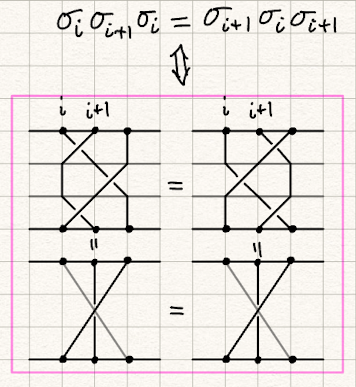
\includegraphics[width = .5\textwidth]{sketch_YB_citerion_verification.png}
    \caption{\colorbox{red}{Grayed-out strand indicates that it is behind all other strands.}}\label{fig:YB_criterion_verification}
\end{figure}

\section{The Burau Representation}
In the previous section, we defined a representation of the braid group $B_n$ as automorphisms of the free group $F_n$. This representation is clearly nonabelian. Likewise, the Artin generators of $B_n$ are nonabelian. Suppose we wish to abelianize the braid group. The details of the abelianization of $B_n$ would require a quotient by the commutator $\left[ a,b \right]=ab\iv{a}\iv{b}$.

Sparing the details, let $B_{n,ab} = B_n/\left[ B_n,B_n \right]$ be the abelianization of $B_n$, where $\left[ B_n,B_n \right]=\left\{ \left[ \beta_1,\beta_2 \right]\st\beta_1,\beta_2\in B_n \right\}$ is the commutator subgroup of $B_n$. Then, under the representation $\rho$ from \cref{sec:Aut_Fn}, the abelianization of \cref{eq:rho_i,eq:rho_ip1,eq:rho_j} become
\begin{align}
    x_i &\xmapsto{\sigma_i} \cancel{x_i} + x_{i+1} - \cancel{x_i} = x_{i+1} = \rho_{\iv{\sigma_i}}(x_i), \\
    x_{i+1} &\xmapsto{\sigma_i} x_i, \\
    x_j &\xmapsto{\sigma_i} x_j, \textrm{ for } j\neq i,i-1,
\end{align}
for each $i$. Thus, the generator $\sigma_i=\iv{\sigma_i}$, and corresponds to a transposition permutation in the symmetric group $S_n$. It follows that $B_{n,ab}\iso S_n$. In this current construction, the abelianization of the braid group results in a loss of complexity. This raises the question whether there exists such a reframing of the braid group that allows an abelian operation on the free generators while preserving the inequivalence of the Artin generators with their inverses.

First, we define a topological space that will aid in the desired construction.
\begin{definition}
    Let $X$ be a topological space. A \textit{covering} of $X$ is a space $\widetilde{X}$ together with a continuous map $p:\widetilde{X}\to X$ such that, for every $x\in X$, there exists a path-connected open neighborhood $U$ containing $x$ such that $\iv{p}(U)$ is a disjoint union of open sets in $\widetilde{X}$ where each component of $\iv{p}(U)$ is mapped homeomorphically onto $U$ by $p$. Each component of $\iv{p}(U)$ is called a \textit{sheet} of the covering, where the $i$-th sheet is denoted by $\sheet{X}{i}$, and total the number of sheets in $\iv{p}(U)$ is called the \textit{degree} of the covering.
\end{definition}

\begin{example}
    One of the simplest examples of a covering space is the covering of the circle $S^1$ by the real line by the parameterization map $p:\R\to S^1$ defined by $p(t)=\left( \cos t,\sin t \right)$. Clearly, there are infinitely many sheets in this covering.
\end{example}

\begin{example}
    A similar example is the covering of the circle $S^1$ through $p:\left[ 0,1 \right]\to S^1$ defined by $p(t) = e^{2\pi it}$. This defines a one-degree covering of $S^1$. If we instead let our domain be $\left[ 0,2 \right]$, then we have a two-degree covering of $S^1$.
\end{example}

With this topological tool, we construct a countably infinite-degree covering of the punctured disk $\D_n$, denoted $\widetilde{\D}_n$, which can be visualized as an infinite stack of copies of $\D_n$, with a slight modification to be explained shortly. Let $\sheet{\D}{n,i}$ denote the $i$-th sheet of $\widetilde{\D}_n$, and consider the base sheet our covering to be $\sheet{\D}{n,0}$.

We start this construction with a countably infinite stack of copies of $\D_n$. Then, for every $i\in\Z$, for each of the $n$ punctures on $\sheet{\D}{n,i}$, apply a cut from the hole to some point on the boundary of $\sheet{\D}{n,i}$, as illustrated in \cref{fig:D3_cuts} for the case when $n=3$. Each cut results in two edges, which will be referred to as the left edge and the right edge. Through a homeomorphic deformation, connect the left edge of $\sheet{\D}{n,i}$ to the corresponding right edge of $\sheet{\D}{n,i+1}$, and the right edge of $\sheet{\D}{n,i}$ to the left edge of $\sheet{\D}{n,i-1}$, for every cut on every sheet.

\begin{figure}[htbp]
    \centering
    % 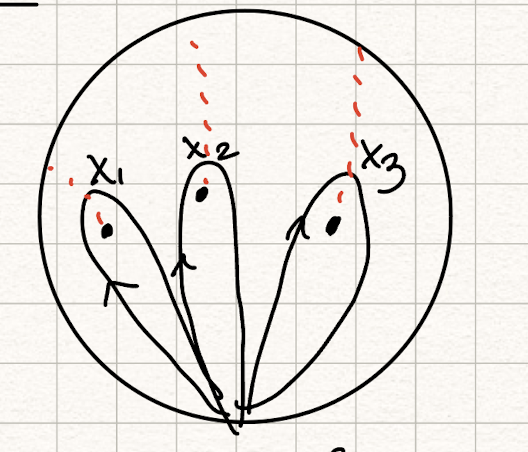
\includegraphics[width=.3\textwidth]{D3_cuts.png}
    % Suggested circle radius >= 3 cm
\usetikzlibrary{
        math,
        calc,
        % decorations.markings,
}

\def\circleRadius{3cm}
\def\sep{\circleRadius*0.175}
% \def\Off{.6}
% \def\eSep{.0005*\circleRadius}
% \def\cSep{1.2*\eSep}
\def\aSep{5} % degrees
\def\lA{130}
\def\cA{90}
\def\rA{50}

\begin{tikzpicture}[
] 
        \node[anchor=north west, font=\Large] at ({-1.15*\circleRadius}, {1.05*\circleRadius}) {$\sheet{\D}{n,i}$};

        \draw[ultra thick] (0,0) circle (\circleRadius);

        \tikzmath{
                coordinate \l, \r, \p, \b, \lI, \lO; real \aL, \aR;
                \aL1 = \lA+\aSep;
                \aR1 = \lA-\aSep;
                \aL2 = \cA+\aSep;
                \aR2 = \cA-\aSep;
                \aL3 = \rA+\aSep;
                \aR3 = \rA-\aSep;
                %
                \b = (0,-\circleRadius);
                \p1 = (-.5*\circleRadius,0);
                \p2 = (0,0);
                \p3 = (.5*\circleRadius,0);
                \l1 = (\aL1:\circleRadius);
                \r1 = (\aR1:\circleRadius);
                \l2 = (\aL2:\circleRadius);
                \r2 = (\aR2:\circleRadius);
                \l3 = (\aL3:\circleRadius);
                \r3 = (\aR3:\circleRadius);
                %
        %         Alternate method with cartesian coordinates
        %         \l1 = ({-(\Off + \eSep)*\circleRadius},{sqrt(1-(\Off + \eSep)^2) * \circleRadius});
        %         \l2 = (-\cSep*\circleRadius,{sqrt(1-(\cSep)^2) * \circleRadius});
        %         \l3 = ({(\Off - \eSep)*\circleRadius},{sqrt(1-(\Off - \eSep)^2) * \circleRadius});
        %         \r1 = ({-(\Off - \eSep)*\circleRadius},{sqrt(1-(\Off - \eSep)^2) * \circleRadius});
        %         \r2 = (\cSep*\circleRadius,{sqrt(1-(\cSep)^2) * \circleRadius});
        %         \r3 = ({(\Off + \eSep)*\circleRadius},{sqrt(1-(\Off + \eSep)^2) * \circleRadius});
        }
        
        % \foreach \i in {1,2,3} {
        %         \draw[white, line width=2pt] (\r\i) arc (atan2(\ry\i,\rx\i):atan2(\ly\i,\lx\i):\circleRadius);
        % }

        \foreach \i in {1,2,3} {
                \draw[white, line width=2pt] (\r\i) arc (\aR\i:\aL\i:\circleRadius);
        }

        % Alternate method with nodes
        % \node (l1) at ({\lA+\aSep}:\circleRadius) {};
        % \node (r1) at ({\lA-\aSep}:\circleRadius) {};
        % 
        % \node (l2) at ({\cA+\aSep}:\circleRadius) {};
        % \node (r2) at ({\cA-\aSep}:\circleRadius) {};
        % 
        % \node (l3) at ({\rA+\aSep}:\circleRadius) {};
        % \node (r3) at ({\rA-\aSep}:\circleRadius) {};

        \foreach \i in {1,2,3} {
                \coordinate (lI\i) at ($(\p\i)!0.5!(\l\i)$);
                \coordinate (lO\i) at ($(\p\i)!0.5!(\r\i)$);

                \fill[cyan] (\l\i) circle (.75pt);
                \fill[purple] (\r\i) circle (.75pt);
        }

        \node at (\l2) [left, yshift=-.3*\circleRadius, xshift=.04*\circleRadius, cyan] {$\substack{\textrm{Left} \\ \textrm{Edge}}$};
        \node at (\r2) [right, yshift=-.3*\circleRadius, xshift=-.04*\circleRadius, purple] {$\substack{\textrm{Right} \\ \textrm{Edge}}$};

        \draw [out=135, in=-140, looseness=.65, line width= 1.4, decoration={markings, mark= at position 0.6 with {\arrow{latex},sloped}}, postaction={decorate}] (\b) to (lI1);
        

        \draw [out=80, in=-170, looseness=.65, line width= 1.4, decoration={markings, mark= at position 0.6 with {\arrowreversed{latex},sloped}}, postaction={decorate}] (\b) to (lI3);

        \draw [out=110, in=-110, looseness=0, ultra thick, cyan] (\p1) to (\l1);
        \draw [out=110, in=-110, looseness=0, ultra thick, cyan] (\p2) to (\l2);
        \draw [out=110, in=-110, looseness=0, ultra thick, cyan] (\p3) to (\l3);
        
        \draw [out=80, in=-80, looseness=0, ultra thick, purple] (\p1) to (\r1);
        \draw [out=80, in=-80, looseness=0, ultra thick, purple] (\p2) to (\r2);
        \draw [out=80, in=-80, looseness=0, ultra thick, purple] (\p3) to (\r3);

        \foreach \i in {1,2,3} {
                \fill[black] (\p\i) circle (2pt);
                \node[above, yshift=-.15*\sep, xshift=.45*\sep] at (\p\i) {$\i$};
        }

        % base point for loop/arrow
        \filldraw [red] (\b) circle (2pt) node[below] {$t^i\zeta$};
\end{tikzpicture}

    \caption{
        % In the case of $\D_3$, this figure demonstrates how the cuts are applied across each of the three punctures for each sheet in the covering $\widetilde{\D}_3$. The power of $t$ in the base point label $t^j\zeta$ indicates that we are on the $j$-th sheet of the covering.
        For the covering of $\D_3$, we observe the $i$-th sheet of $\widetilde{\D}_3$ with the cuts applied across each of the three punctures. The base point of the loop is indicated by the red dot, and labelled as $t^i\zeta$. The power of $t$ indicates that we are on the $i$-th sheet of the covering. The portions of three different loops are drawn to illustrate the behavior of loops as they pass through various edges on $\sheet{\D}{3,i}$. The loop that would traditionally be $x_1$ is labeled by $t^i x_1$ to indicate that it's starting on the $i$-th sheet. When it passes through the left edge corresponding to this puncture labeled with a 1, it traverses up to the sheet $\sheet{\D}{3,i+1}$ and ends at base point $t^{i+1}\zeta$. Similarly, the loop that started on $\sheet{\D}{3,i-1}$ and passed through the left edge of puncture 2 ends up coming out of the right edge of puncture 2 on $\sheet{\D}{3,i}$ and ends at the base point $t^i\zeta$. This loop is labeled by the starting sheet, so it is $t^{i-1}x_2$. Finally, the loop that started on $\sheet{\D}{3,i+1}$ and passed through the right edge of puncture 3 ends up coming out of the left edge of puncture 3 on $\sheet{\D}{3,i}$ and is therefore labeled by $-t^{i+1}x_3$, with the negative sign indicating that the loop direction is reversed.
    }\label{fig:D3_cuts}
\end{figure}

Now, viewing a single sheet, say $\sheet{\D}{n,0}$, from above, when a loop with base point $\tilde{\zeta}_0$ passes through a cut from the left, it traverses up to the next sheet, and ends at the base point $\tilde{\zeta}_1$. Similarly, a loop passing through a cut from the right ends at the base point $\tilde{\zeta}_{-1}$, on the sheet $\sheet{\D}{n,-1}$ below $\sheet{\D}{n,0}$. To keep track of the starting sheet of a loop, we use a free parameter $t$. For example, a loop $\gamma$ that starts on $\sheet{\D}{n,j}$ would be written $t^j \gamma$, for $j\in\Z$. Notice that the substitution of a complex number for the free parameter $t$ results in a possibly finite degree covering. As an example, if we set $t$ to an $n$-th root of unity, then we obtain an $n$-th degree covering of $\D_n$. For the purposes of this construction, we will keep $t$ as a free parameter for now.{ }\cref{fig:D3_cuts} demonstrates how loops interact with the cuts on different sheets. The following example describes the action of the standard generators of $B_3$ on the covering space $\widetilde{\D}_3$.

\begin{example}\label{ex:Burau_D3}
    Consider the case when $n=3$. Then we have the corresponding covering space $\widetilde{\D}_3$ of $\D_3$. See \cref{fig:D3_cuts} for the view of a single sheet with various loops interacting with the cuts on the sheet. The actions of the standard generators of $B_3$ in $\pi_1(\D_3)$ are known, and can be visually understood in \cref{fig:sigma_on_Dn}. In the context of the covering space $\widetilde{\D}_3$, the action of the generators $\sigma_1$ and $\sigma_2$ is observed by reducing the visualization to only the base points on each sheet and the loops themselves. This can be seen in \cref{fig:Burau_D3} for the case of $\sigma_1$.
    
    \begin{figure}[htbp]
        \centering
        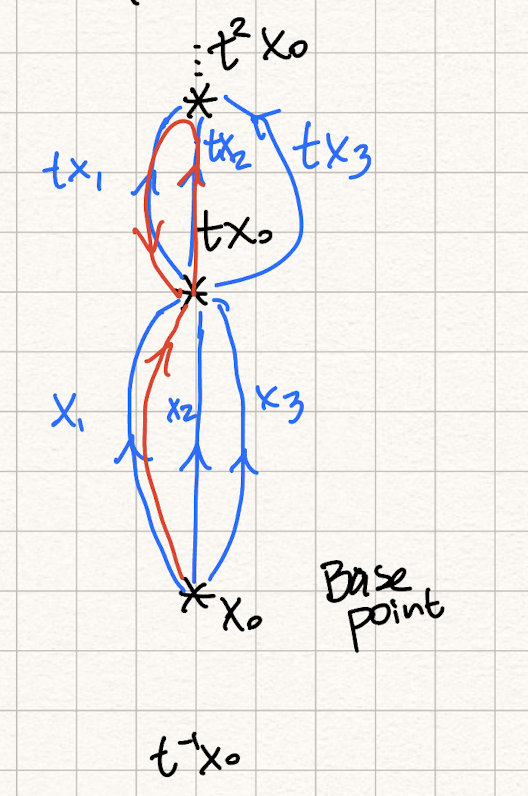
\includegraphics[width = .3\textwidth]{Burau_D3.png}
    %     % \input{TikZ/D3_covering.tikz}
        \caption{\colorbox{red}{CAPTION}}\label{fig:Burau_D3}
    \end{figure}

    Now, we can express loop concatenation as an abelian operation, where \cref{eq:rho_i,eq:rho_ip1,eq:rho_j} become
    \begin{align}
        x_1 \xmapsto{\sigma_1} x_1 + tx_2 - tx_1 &= (1-t)x_1 + tx_2, \\
        x_{2} &\xmapsto{\sigma_1} x_1, \\
        x_3 &\xmapsto{\sigma_1} x_3.
    \end{align}
    Consider the vector $\begin{bmatrix}
        x_1 \\ x_2 \\ x_3
    \end{bmatrix}$. Then the action of $\sigma_1$ on the loops $x_1,x_2,x_3$ is realized by the matrix $\begin{bmatrix}
        1-t & t & 0 \\ 1 & 0 & 0 \\ 0 & 0 & 1
    \end{bmatrix}$ since
    \begin{equation}
        \begin{bmatrix}
            1-t & t & 0 \\ 1 & 0 & 0 \\ 0 & 0 & 1
        \end{bmatrix}\begin{bmatrix}
            x_1 \\ x_2 \\ x_3
        \end{bmatrix} = \begin{bmatrix}
            (1-t)x_1 + tx_2 \\ x_1 \\ x_3
        \end{bmatrix}.
    \end{equation}
    The action of $\sigma_2$ is obtained similarly, where
    \begin{equation}
        \sigma_2 \mapsto \begin{bmatrix}
            1 & 0 & 0 \\ 0 & 1-t & t \\ 0 & 1 & 0
        \end{bmatrix}.
    \end{equation}
    Notice that these matrices have entries in the ring of Laurent polynomials, $\Lambda=\Z[t,\iv{t}]$.
\end{example}

Clearly, the result from \cref{ex:Burau_D3} generalizes to the case of braids on $n$ strands. Fix $n>1$. Let $I_k$ denote the $k\times k$ dimensional identity matrix, and let
\begin{equation}
    U=\begin{bmatrix}
        1-t & t \\ 1 & 0
    \end{bmatrix}.
\end{equation} 
For $i\in\left\{ 1,\dots,n-1 \right\}$, the action of $\sigma_i$ on $\pi_1\left( \widetilde{\D}_n \right)$ is realized as an $n\times n$ matrix with entries in $\Lambda = \Z[t,\iv{t}]$. 

The Burau representation of $B_n$ is then defined by:
\begin{align}
    \psi_n:B_n&\to\textrm{GL}_n(\Lambda) \\
    \sigma_i &\mapsto \begin{bmatrix}
        I_{i-1} & 0 & 0 \\
        0 & U & 0 \\
        0 & 0 & I_{n-i-1}
    \end{bmatrix}.
\end{align}
\colorbox{red}{Show invertible/inverse?}

The Burau representation need only be defined on the standard generators, since any braid $\beta\in B_n$ decomposes into a product of $\sigma_1,\dots,\sigma_{n-1}$ and their inverses. Notice that if we set $t\to 1$, we recover the defining representation of $S_n$, as expected when we use a degree 1 covering space of $\D_n$ and force the action of the generators to be abelian. Furthermore, by direct computation, it follows that
\begin{align}
    \psi_n(\sigma_i)\psi_n(\sigma_j) &= \psi_n(\sigma_j)\psi_n(\sigma_i) \textrm{ for } |i-j|>1, \\
    \psi_n(\sigma_i)\psi_n(\sigma_{i+1})\psi_n(\sigma_i) &= \psi_n(\sigma_{i+1})\psi_n(\sigma_i)\psi_n(\sigma_{i+1}) \textrm{ for } |i-j|=1.
\end{align}

\chapter{tikz test}\label{ch:tikz_test}

\begin{figure}[htbp]
    \centering
    \def\circleRadius{2.5cm}
\def\sep{\circleRadius*0.175}
\def\XOff{1.5*\circleRadius}
\def\YOff{-2.5*\circleRadius}

\pgfdeclarelayer{edgelayer}
\pgfdeclarelayer{nodelayer}
\pgfsetlayers{edgelayer,nodelayer,main}

\newcommand{\drawRegion}[3]{
        \begin{scope}[shift={#1}]
        \node[anchor=north west, font=\large] at (-\circleRadius, \circleRadius) {$\D_n$};

        \draw[ultra thick] (0,0) circle (\circleRadius);
        \filldraw [black] 
                (-\circleRadius + \sep,0) circle (2pt) node[above] {$1$}
                (\circleRadius - \sep,0) circle (2pt) node[above] {$n$}
                (-\sep,0) circle (2pt) node[above, yshift=.2*\sep] {$i$}
                (\sep,0) circle (2pt) node[above, yshift=.1*\sep] {$i+1$};
        \path (-\circleRadius/2,0) node {$\scalebox{1.5}{$\cdots$}$};
        \path (\circleRadius/2,0) node {$\scalebox{1.5}{$\cdots$}$};

        \ifx&#2&  % Check if #2 is empty
                % Do nothing if #2 is empty
        \else
                \draw[-latex, ultra thick] (0,-\circleRadius) .. controls #2 .. node[pos=0.1, left] {#3} (.05*\sep,-\circleRadius + 2.8452755906/2);
        \fi
        
        \filldraw [red] (0,-\circleRadius) circle (2pt);
        
        \end{scope}
}


\begin{tikzpicture}
        \drawRegion{(\XOff,0)}{(-1.425*\sep-.35*\circleRadius,0.39*\circleRadius) and  (-1.425*\sep+.35*\circleRadius,0.39*\circleRadius)}{$x_i$}
        
        \draw[-latex, ultra thick] (-\XOff + \circleRadius + 0.25cm, 0) -- node[above] {$\sigma_i$} (\XOff - \circleRadius - 0.25cm, 0);
        
        \drawRegion{(-\XOff,0)}{(1.3*\sep-.35*\circleRadius,0.39*\circleRadius) and  (1.3*\sep+.35*\circleRadius,0.39*\circleRadius)}{$x_{i+1}$}
        
        \drawRegion{(-\XOff,\YOff)}{(-1.425*\sep-.35*\circleRadius,0.39*\circleRadius) and  (-1.425*\sep+.35*\circleRadius,0.39*\circleRadius)}{$x_i$}

        \draw[-latex, ultra thick] (-\XOff + \circleRadius + 0.25cm, \YOff) -- node[above] {$\sigma_i$} (\XOff - \circleRadius - 0.25cm, \YOff);
        
        % \drawRegion{(\XOff,\YOff)}{}{}

        \begin{scope}[shift={(\XOff,\YOff)}]
                \node[anchor=north west, font=\large] at (-\circleRadius, \circleRadius) {$\D_n$};
        
                \draw[ultra thick] (0,0) circle (\circleRadius);
                \filldraw [black] 
                        (-\circleRadius + \sep,0) circle (2pt) node[above] {$1$}
                        (\circleRadius - \sep,0) circle (2pt) node[above] {$n$}
                        (-\sep,0) circle (2pt) node[above, yshift=.45*\sep] {$i$}
                        (\sep,0) circle (2pt) node[above, yshift=.3*\sep] {$i+1$};
                \path (-\circleRadius/2,0) node {$\scalebox{1.5}{$\cdots$}$};
                \path (\circleRadius/2,0) node {$\scalebox{1.5}{$\cdots$}$};
        
                \filldraw [red] (0,-\circleRadius) circle (2pt);

                \begin{pgfonlayer}{nodelayer}
                        \node (0) at (-1.5*\sep,.35*\sep ) {};
                        \node (1) at (0, -\circleRadius) {};
                        \node (2) at (1.5*\sep, -1.5*\sep) {$x_i x_{i+1}\iv{x_i}$};
                        \node (3) at (1.25*\sep, -.25*\sep) {};
                        \node (4) at (-.5*\sep, .35*\sep) {};
                        \node (5) at (.05*\sep, -\circleRadius + 2.8452755906/2) {};
                \end{pgfonlayer}
                \begin{pgfonlayer}{edgelayer}
                        \draw [in=105, out=-120, looseness=0.50, ultra thick] (0.center) to (1.center);
                        \draw [in=60, out=30, looseness=0.85, ultra thick] (3.center) to (0.center);
                        \draw [in=-150, out=-15, looseness=0.50, ultra thick] (4.center) to (3.center);
                        \draw [latex-, in=165, out=85, ultra thick] (5.center) to (4.center);
                \end{pgfonlayer}

                % \foreach \point in {0,1,3,4,5} {
                %         \fill[red] (\point) circle (2pt);
                %         \node[above right] at (\point) {\point};
                % }
        \end{scope}
        
        \draw[-latex, ultra thick] (-\XOff + \circleRadius + 0.25cm, 0) -- node[above] {$\sigma_i$} (\XOff - \circleRadius - 0.25cm, 0);
\end{tikzpicture}
\end{figure}

\addcontentsline{toc}{chapter}{References}
\nocite{*} % Include all references in the bibliography
% Bibliography with hyperlinks
\hypersetup{
    linkcolor=blue,
    citecolor=blue,
    urlcolor=blue
}
\bibliographystyle{plain}
\bibliography{references}

\end{document}